\section{Korrelationsmatrizen sortiert nach der Bevölkerungsdichte}
\subsection{Korrelationsmatrizen mit den nach Bevölkerungsdichten sortierten Landkreisen}
In \autoref{fig:matrizes_pop_density_counties} finden sich die sechs Matrizen mit den Werten für die Korrelationen zwischen allen Landkreisen. Die Zeilen und Spalten sind nach der Bevölkerungsdichte der Landkreise sortiert, eine vollständige Auflistung befindet sich im Anhang in \autoref{tab:counties_by_pop_density}.

\subsection{Korrelationsmatrizen mit den nach Bevölkerungsdichten sortierten Regierungsbezirken}
In \autoref{fig:matrizes_pop_density_districts} finden sich die sechs Matrizen mit den Werten für die Korrelationen zwischen den Regierungsbezirken. Die Zeilen und Spalten sind nach der Bevölkerungsdichte der Regierungsbezirke sortiert, eine vollständige Auflistung befindet sich im Anhang in \autoref{tab:districts_by_pop_density}.

\begin{figure}[H]
    \centering
    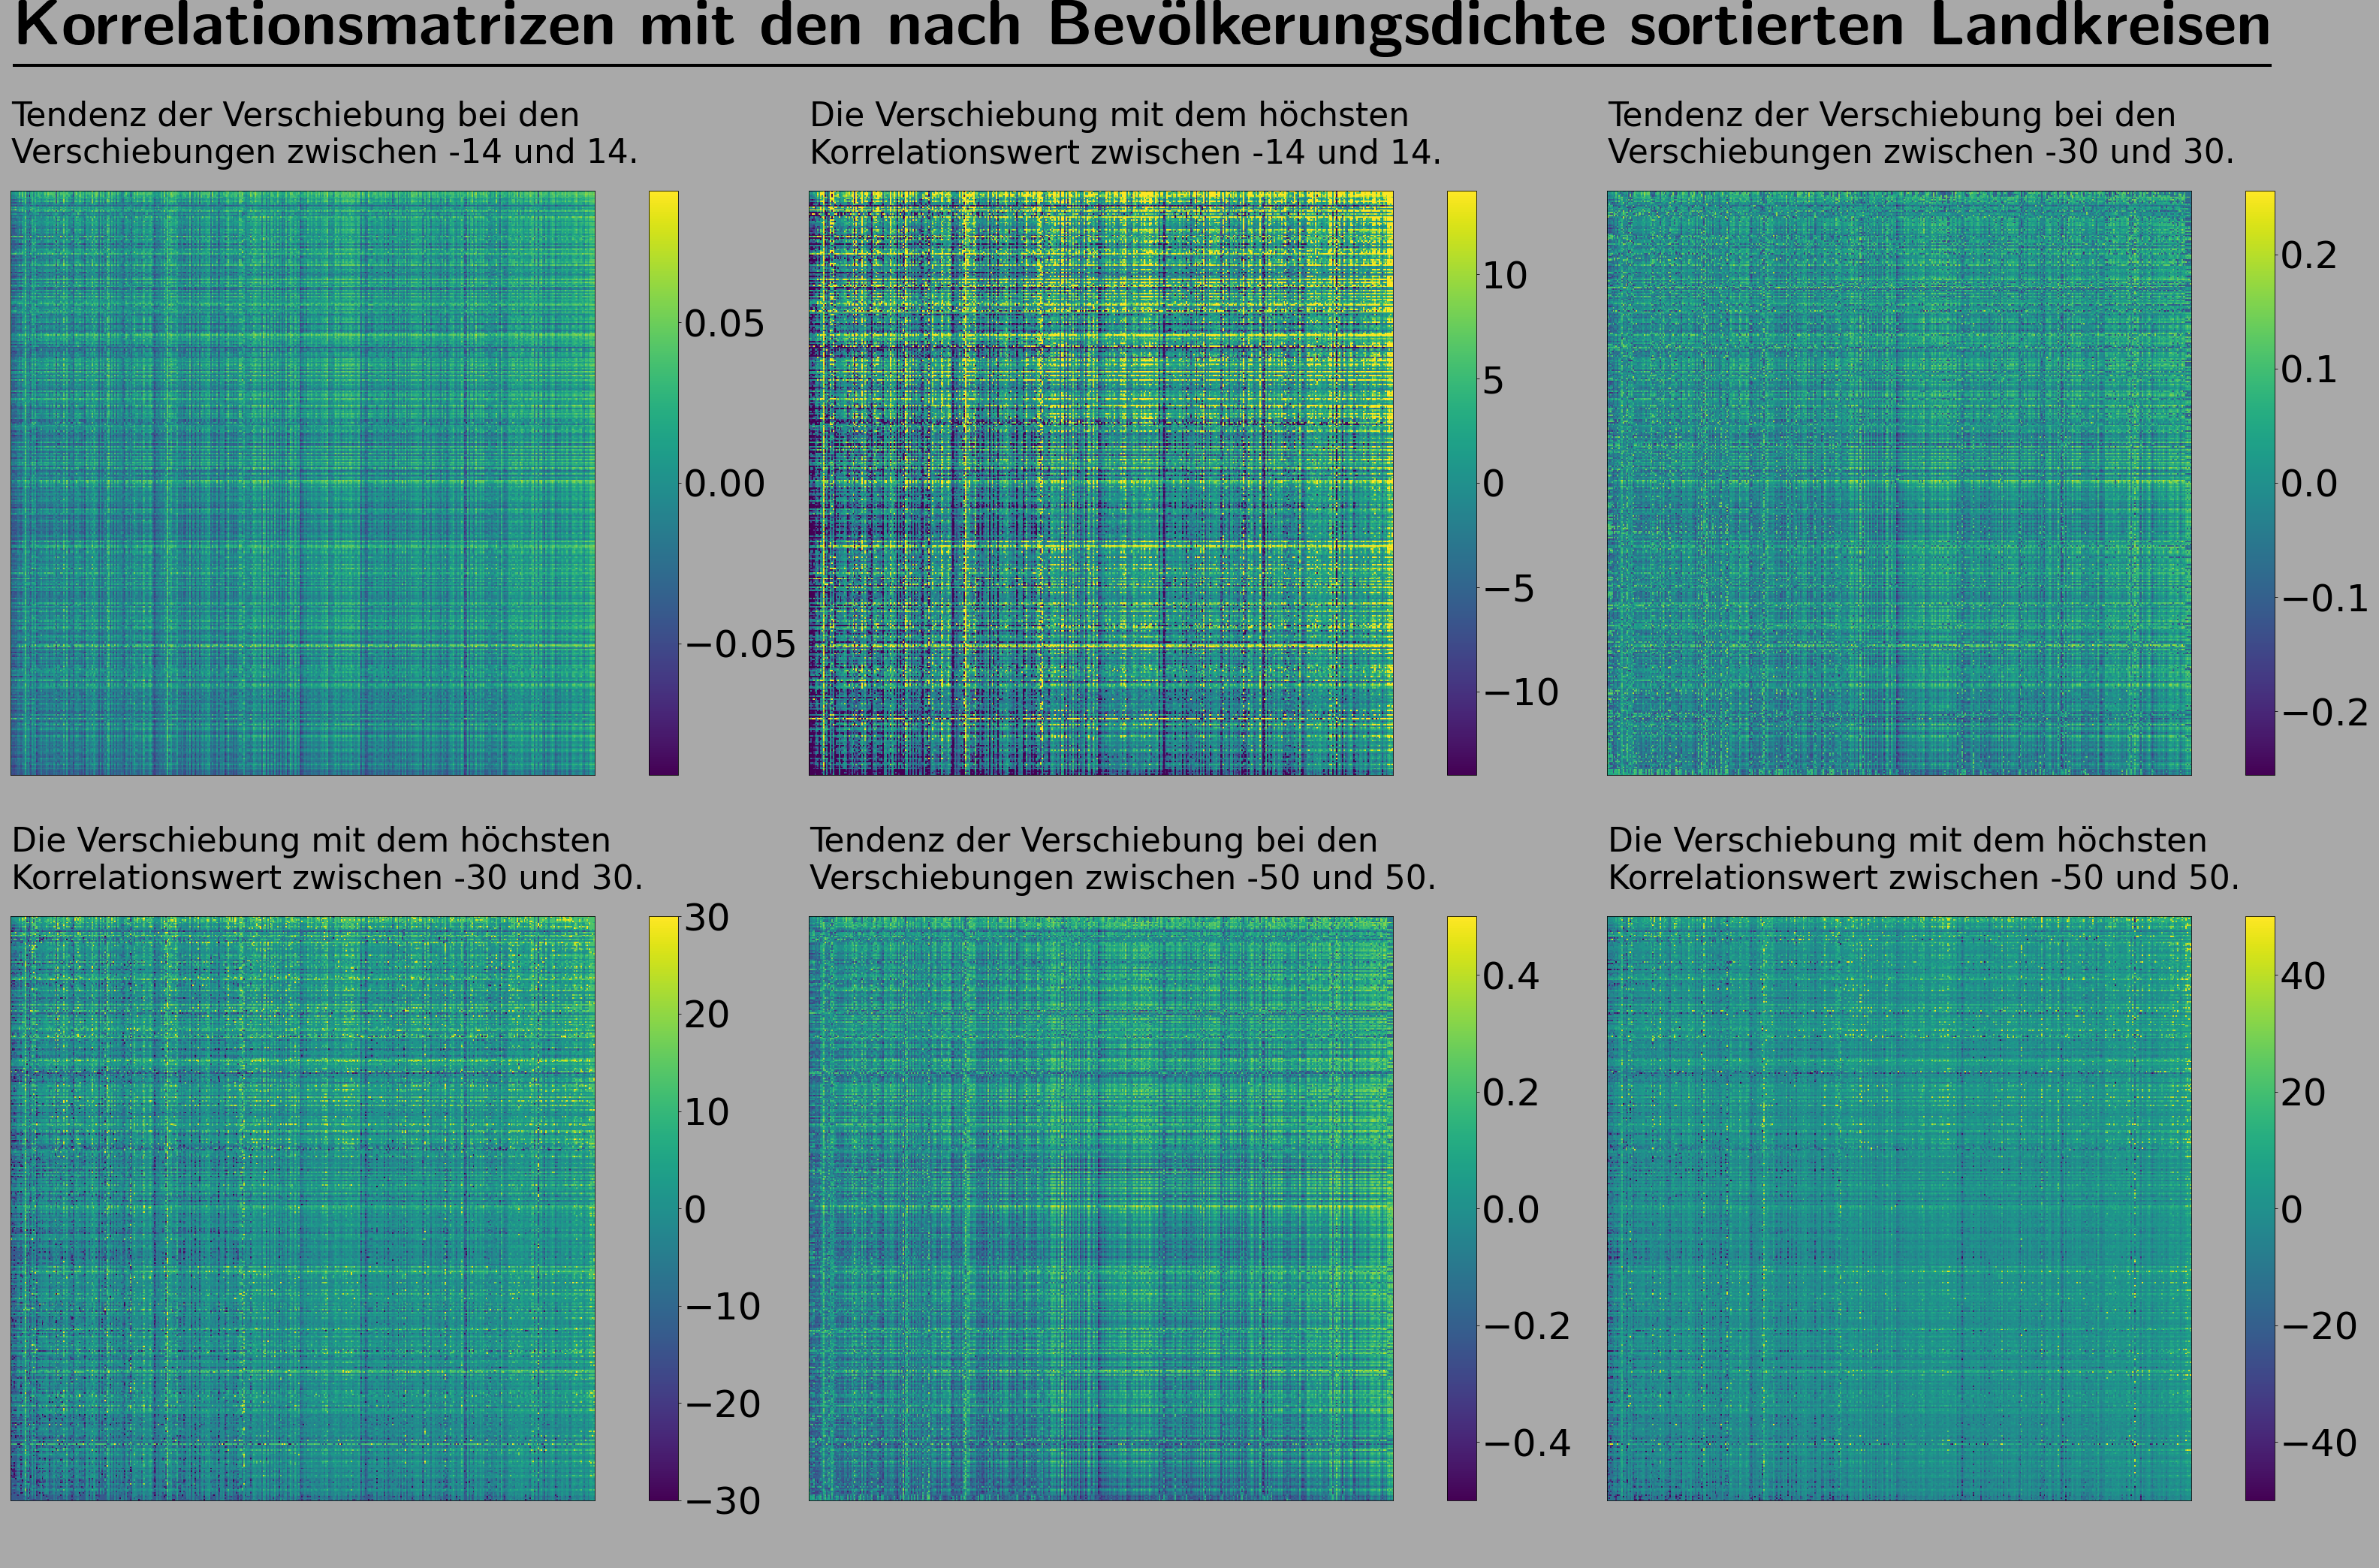
\includegraphics[width = 0.75\textwidth]{figures/Ergebnisse/matrizes_pop_density_counties.png}
    \caption{Korrelationsmatrizen der Korrelationen aller Landkreise zeilen- und spaltenweise nach der Bevölkerungsdichte sortiert (siehe \autoref{tab:counties_by_pop_density}). Die Farben der Zellen der linken Matrizen entsprechen den Tendenzen der Verschiebung des Landkreises der Spalte in Relation zum Landkreis der Zeile.
    Auf der rechten Seite wir die Zelle entsprechend der Verschiebung der Zeitserie des Landkreises der Spalte entgegen der Zeitserie der Zeile mit dem höchsten Korrelationswert eingefärbt. Beide Vorgehensweise werden für alle ganzzahligen Verschiebungen $\tau\in[-14,14]$,  $\tau\in[-30,30]$ und  $\tau\in[-50,50]$ durchgeführt und in dieser Reihenfolge von oben nach unten dargestellt.}
    \label{fig:matrizes_pop_density_counties}
\end{figure}

\begin{figure}[H]
    \centering
    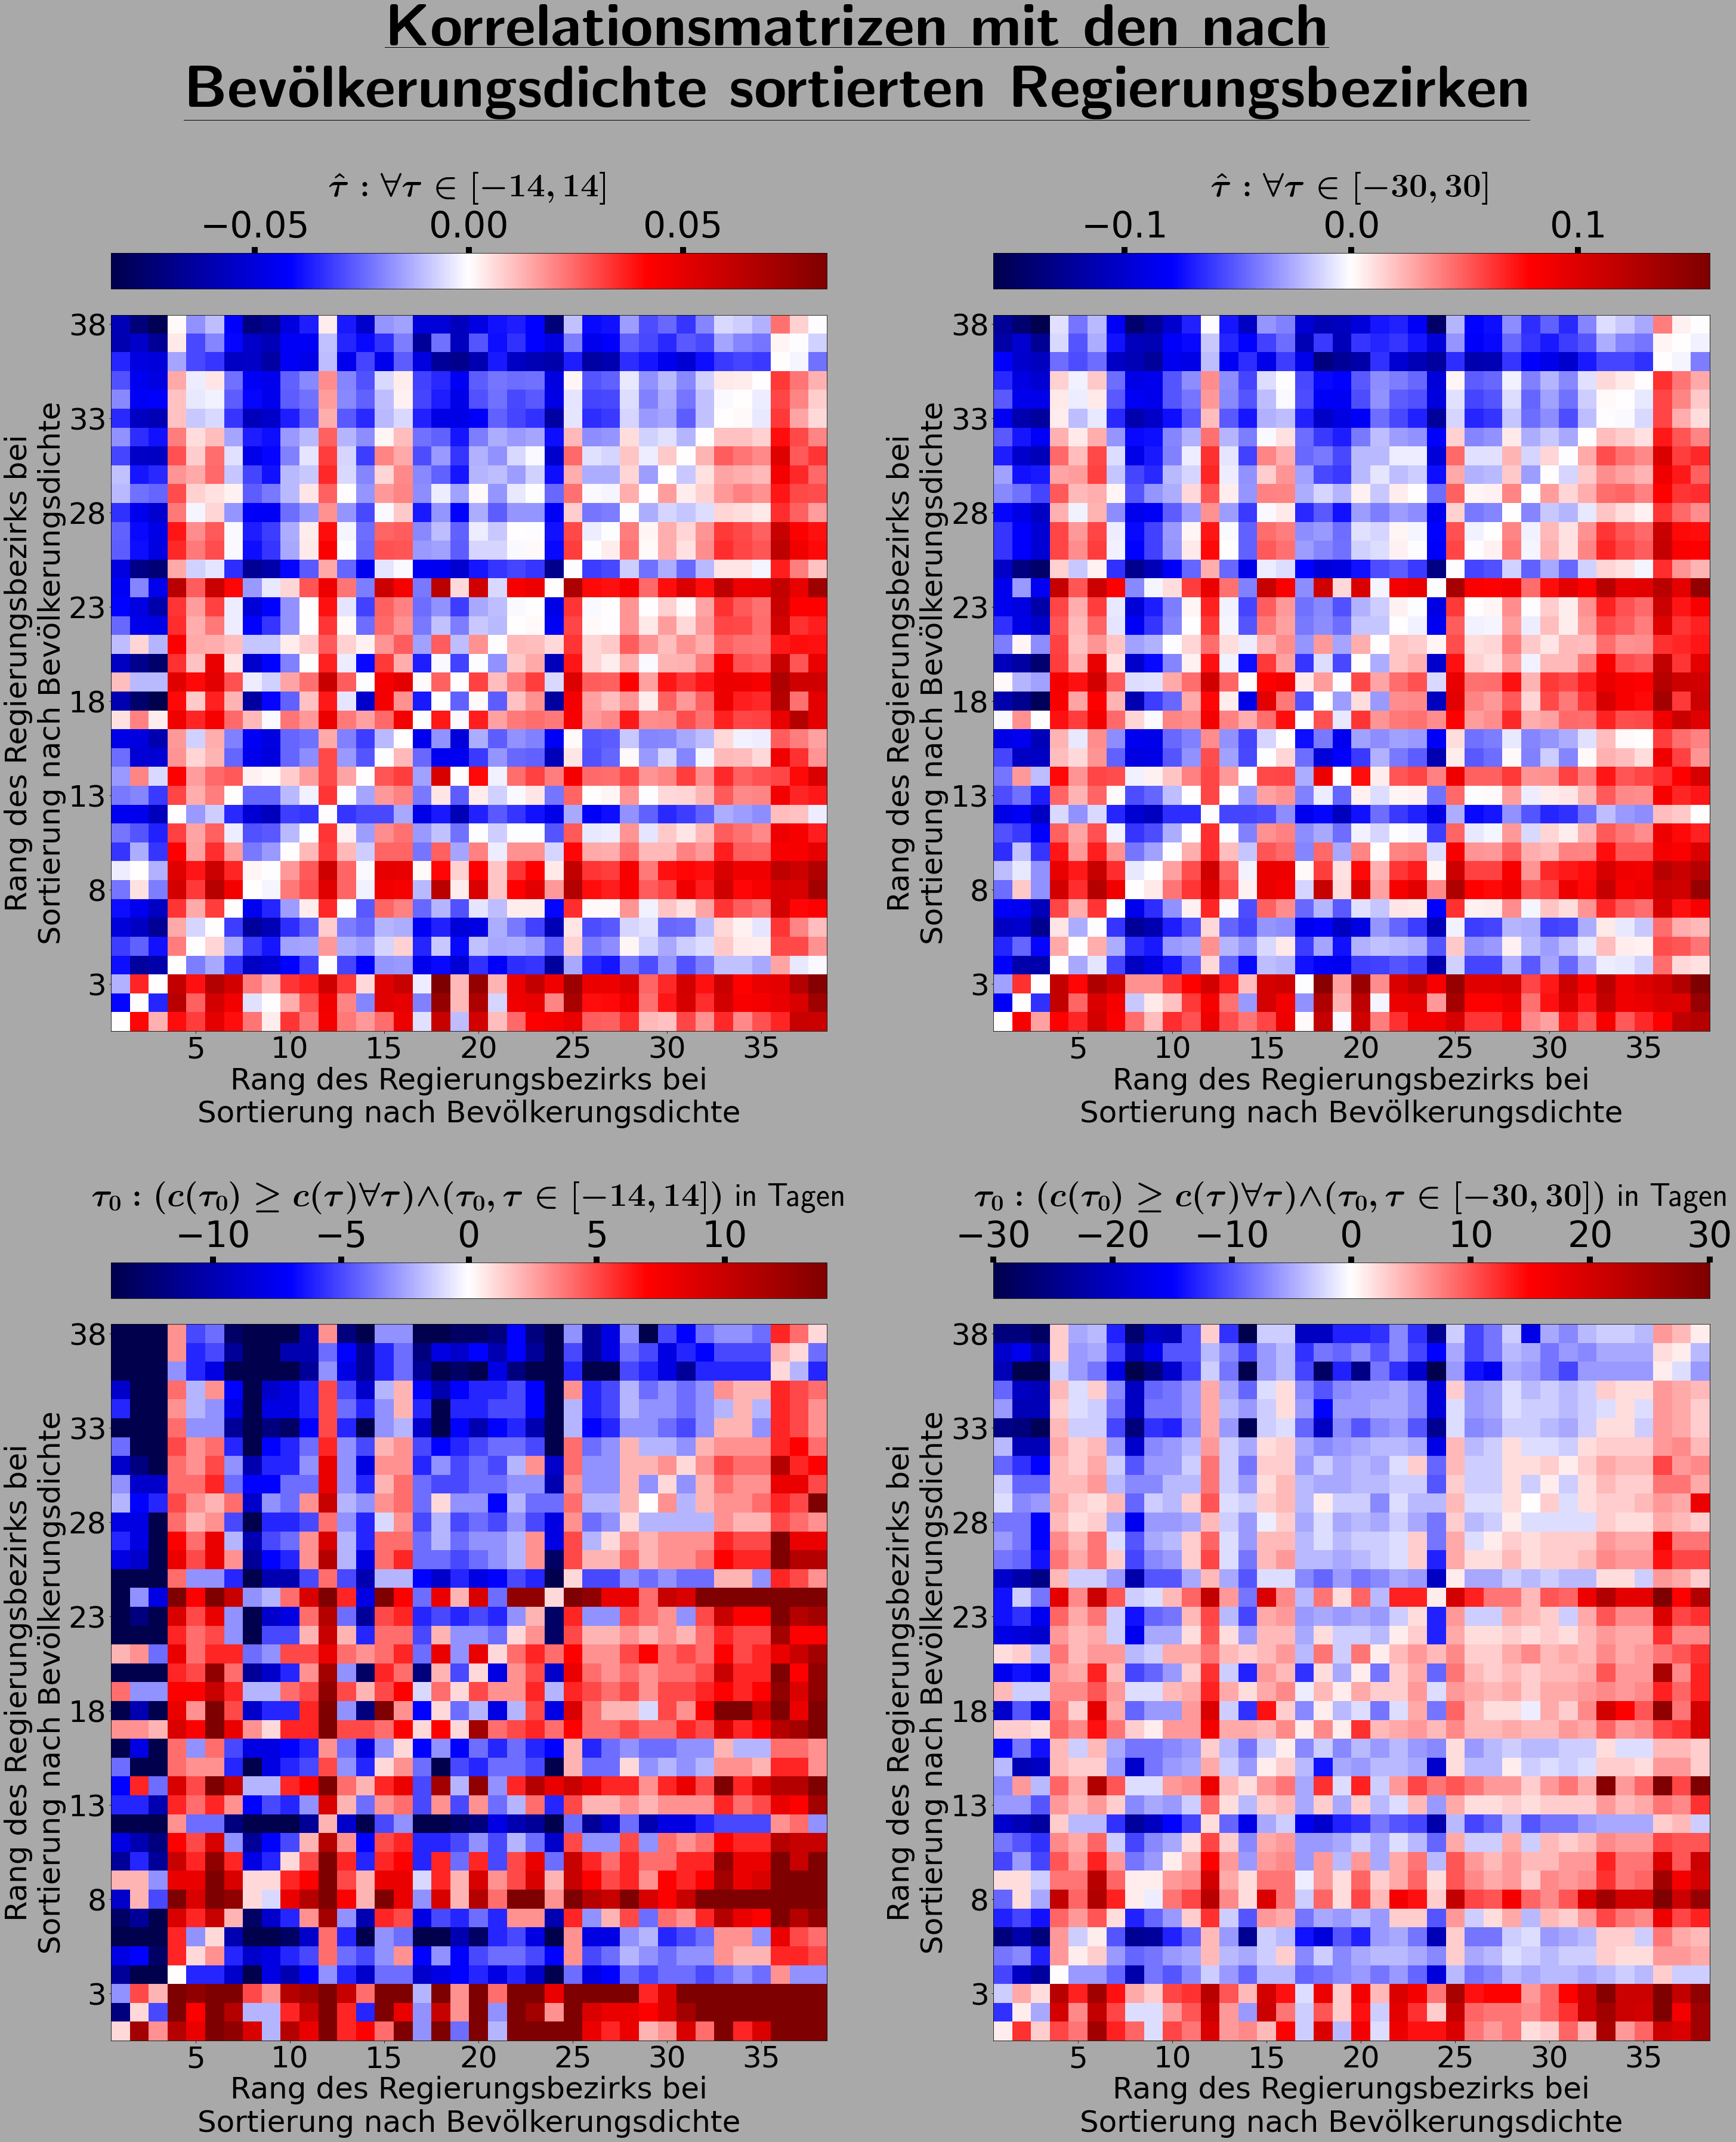
\includegraphics[width = 0.75\textwidth]{figures/Ergebnisse/matrizes_pop_density_districts.png}
    \caption{Korrelationsmatrizen der Korrelationen aller Regierungsbezirke zeilen- und spaltenweise nach der Bevölkerungsdichte sortiert (siehe \autoref{tab:districts_by_pop_density}). Die Farben der Zellen der linken Matrizen entsprechen den Tendenzen der Verschiebung des Regierungsbezirks der Spalte in Relation zum Regierungsbezirks der Zeile.
    Auf der rechten Seite wir die Zelle entsprechend der Verschiebung der Zeitserie des Regierungsbezirks der Spalte entgegen der Zeitserie der Zeile mit dem höchsten Korrelationswert eingefärbt. Beide Vorgehensweise werden für alle ganzzahligen Verschiebungen $\tau\in[-14,14]$,  $\tau\in[-30,30]$ und  $\tau\in[-50,50]$ durchgeführt und in dieser Reihenfolge von oben nach unten dargestellt.}
    \label{fig:matrizes_pop_density_districts}
\end{figure}

